\appendix

\section{Mental models}

\begin{figure*}[ht]
	\centering

	\begin{subfigure}[t]{.45\linewidth}
		\centering
		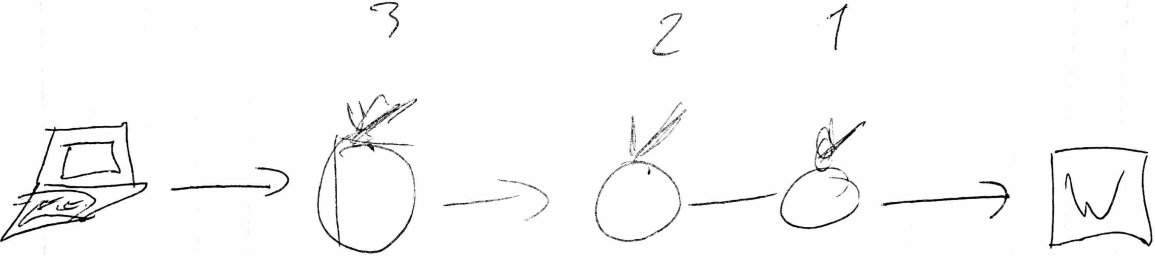
\includegraphics[width=\linewidth]{figures/p01-tor-sketch.jpg}
		\subcaption{Tor sketch.}
		\label{fig:p01-tor-sketch}
	\end{subfigure}
	\hfill
	\begin{subfigure}[t]{.45\linewidth}
		\centering
		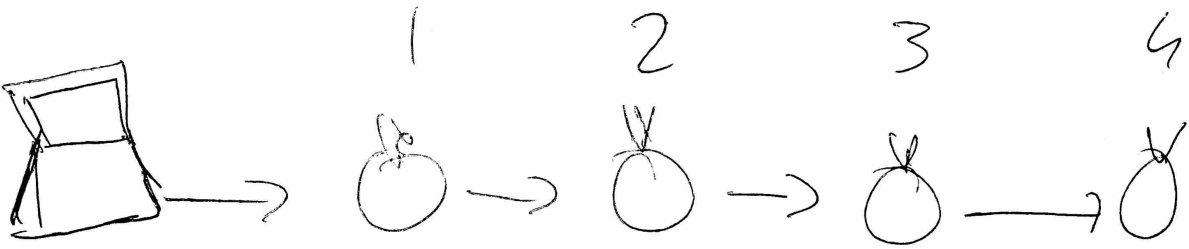
\includegraphics[width=\linewidth]{figures/p01-os-sketch.jpg}
		\subcaption{Onion service sketch.}
		\label{fig:p01-os-sketch}
	\end{subfigure}

	\begin{subfigure}[t]{.45\linewidth}
		\centering
		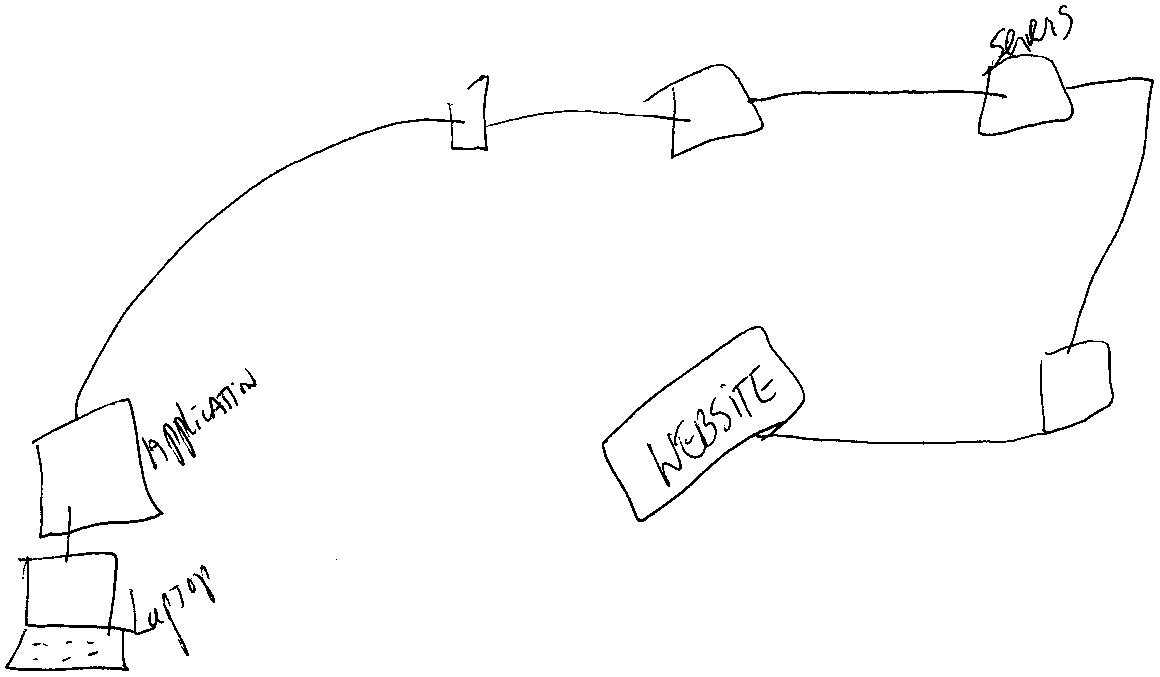
\includegraphics[width=\linewidth]{figures/p02-tor-sketch.jpg}
		\subcaption{Tor sketch.}
		\label{fig:p02-tor-sketch}
	\end{subfigure}
	\hfill
	\begin{subfigure}[t]{.45\linewidth}
		\centering
		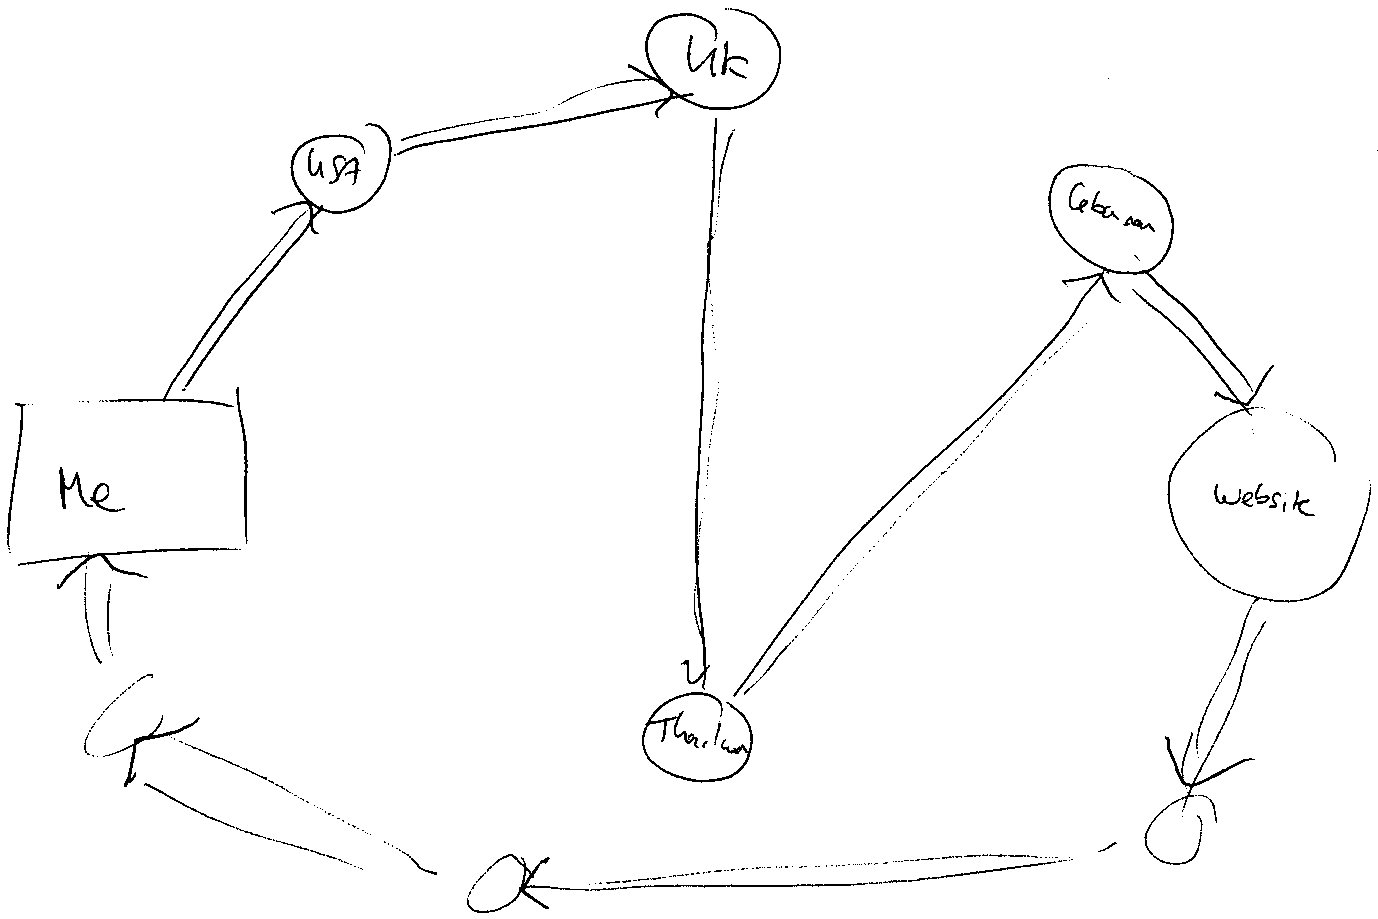
\includegraphics[width=\linewidth]{figures/p03-tor-sketch.jpg}
		\subcaption{Tor sketch.}
		\label{fig:p03-tor-sketch}
	\end{subfigure}

	\begin{subfigure}[t]{.45\linewidth}
		\centering
		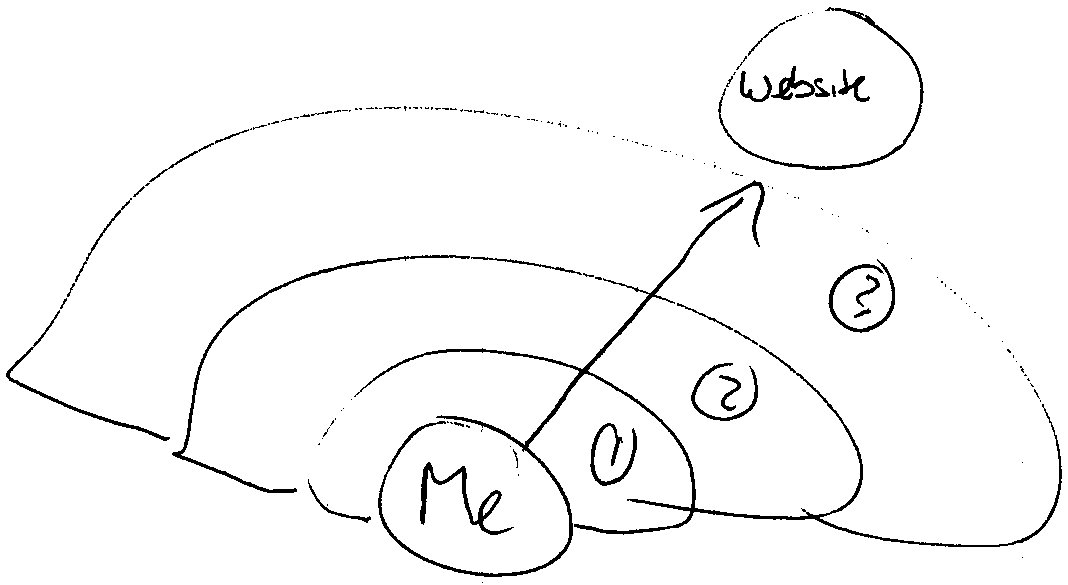
\includegraphics[width=\linewidth]{figures/p03-os-sketch.jpg}
		\subcaption{Onion service sketch.}
		\label{fig:p03-os-sketch}
	\end{subfigure}
	\hfill
	\begin{subfigure}[t]{.45\linewidth}
		\centering
		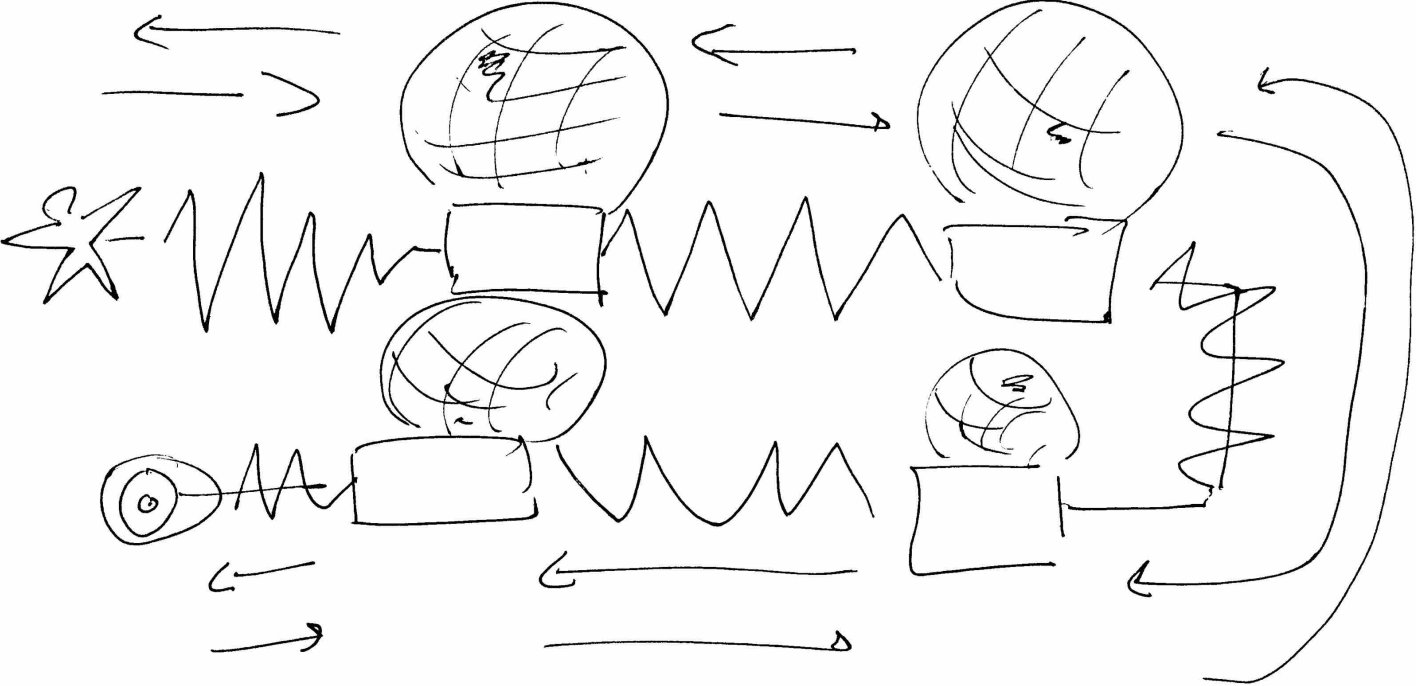
\includegraphics[width=\linewidth]{figures/p04-tor-sketch.jpg}
		\subcaption{Tor sketch.}
		\label{fig:p04-tor-sketch}
	\end{subfigure}

	\begin{subfigure}[t]{.45\linewidth}
		\centering
		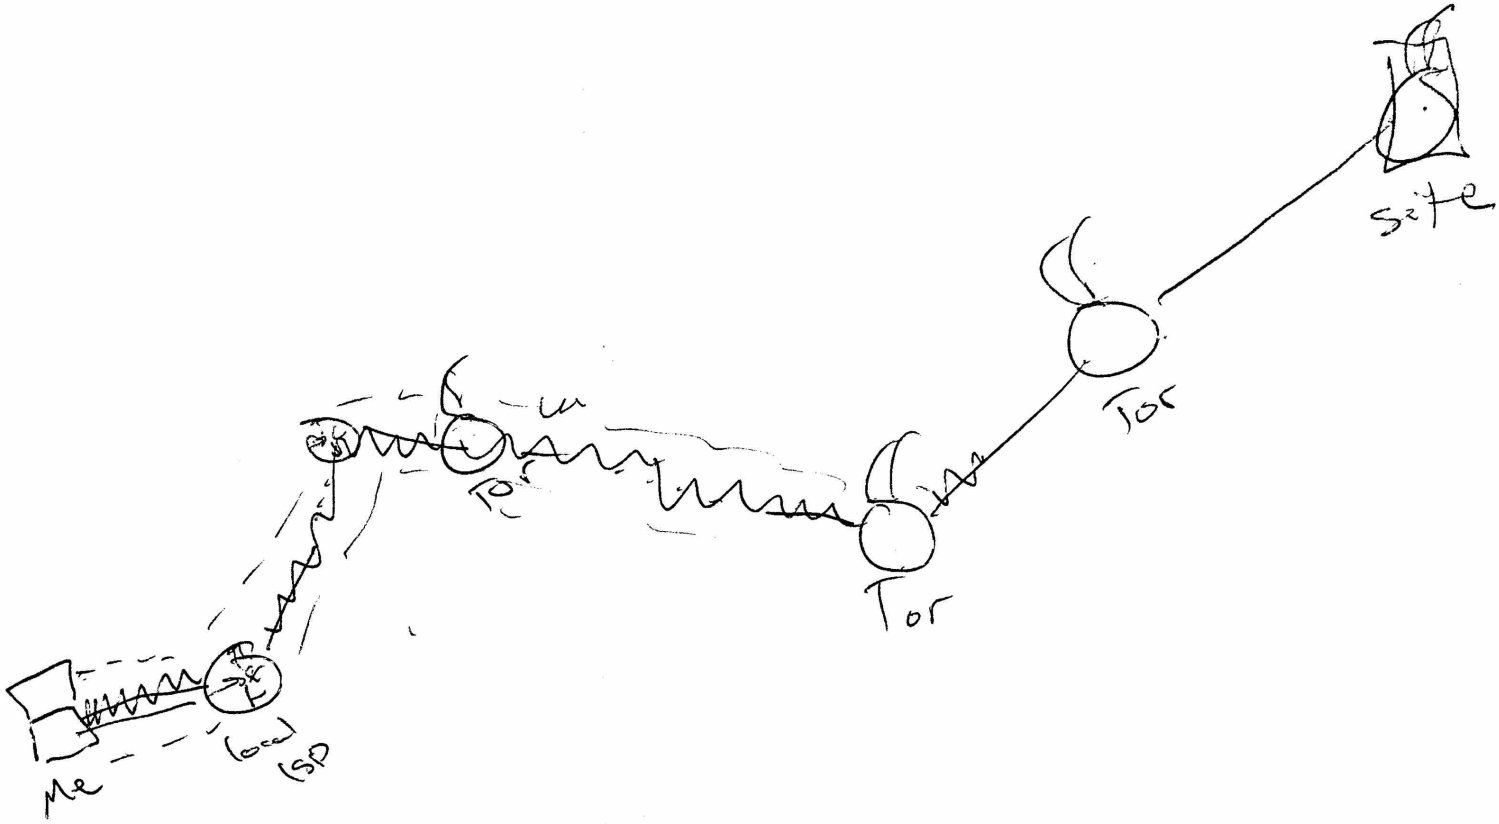
\includegraphics[width=\linewidth]{figures/p05-tor-sketch.jpg}
		\subcaption{Tor sketch.}
		\label{fig:p05-tor-sketch}
	\end{subfigure}
	\hfill
	\begin{subfigure}[t]{.45\linewidth}
		\centering
		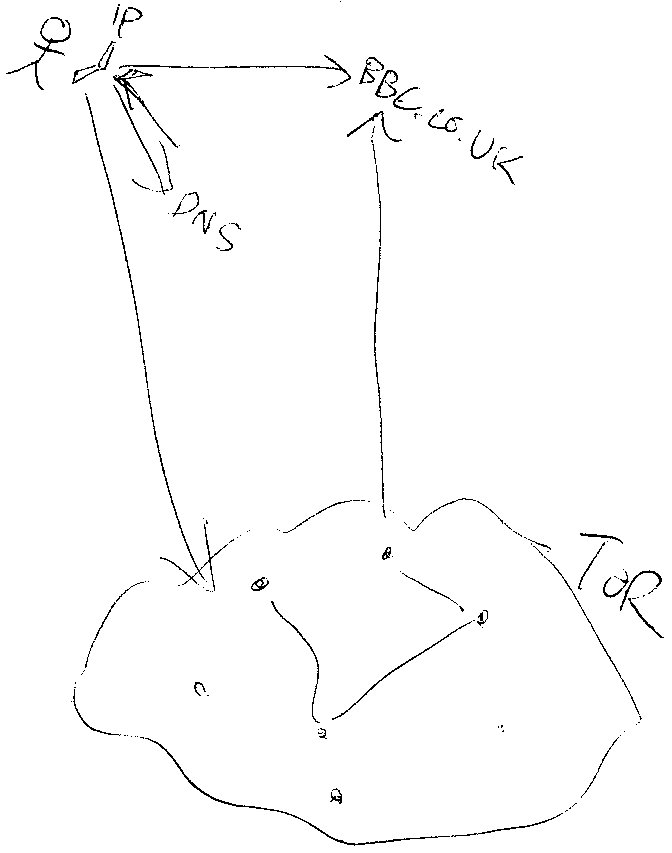
\includegraphics[width=.6\linewidth]{figures/p06-tor-sketch.jpg}
		\subcaption{Tor sketch.}
		\label{fig:p06-tor-sketch}
	\end{subfigure}

	\caption{Bla.}
\end{figure*}

\begin{figure*}[ht]\ContinuedFloat
	\centering

	\begin{subfigure}[t]{.45\linewidth}
		\centering
		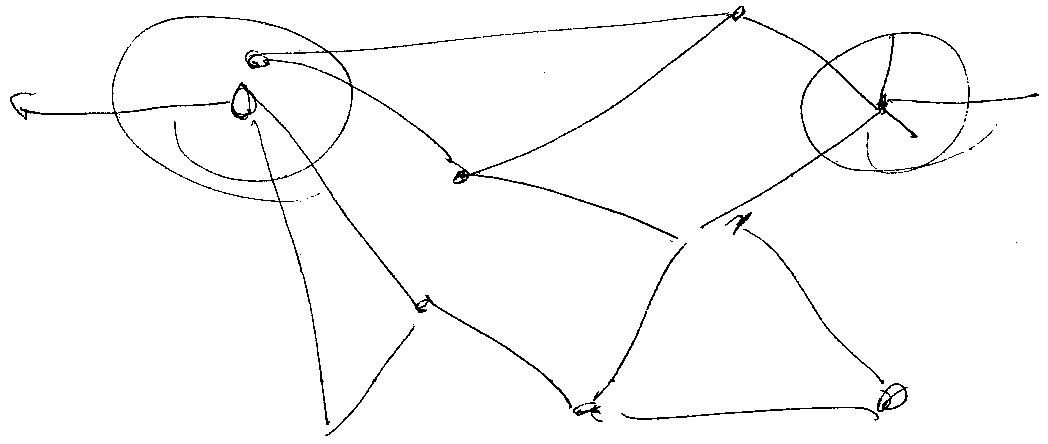
\includegraphics[width=\linewidth]{figures/p07-tor-sketch.jpg}
		\subcaption{Tor sketch.}
		\label{fig:p07-tor-sketch}
	\end{subfigure}
	\hfill
	\begin{subfigure}[t]{.45\linewidth}
		\centering
		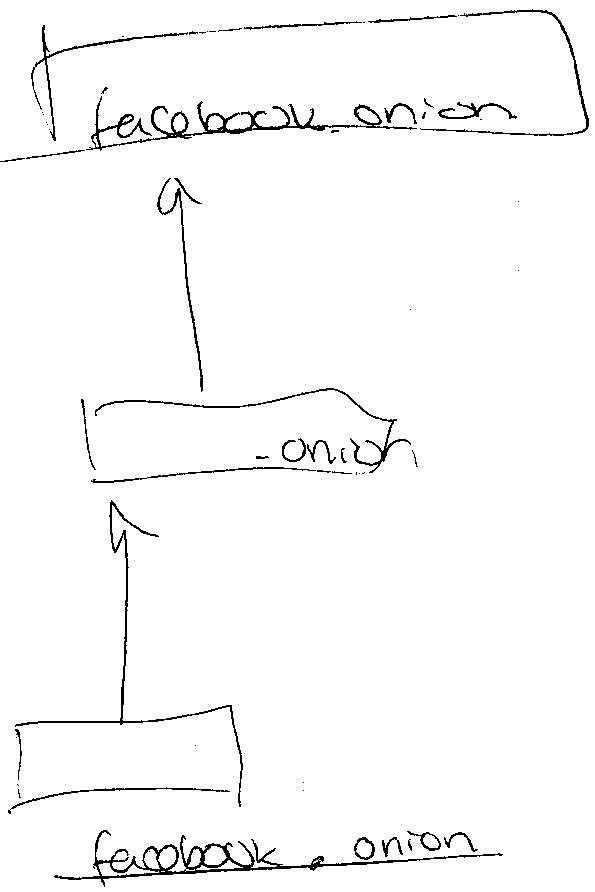
\includegraphics[width=.4\linewidth]{figures/p07-os-sketch.jpg}
		\subcaption{Onion service sketch.}
		\label{fig:p07-os-sketch}
	\end{subfigure}

	\begin{subfigure}[t]{.45\linewidth}
		\centering
		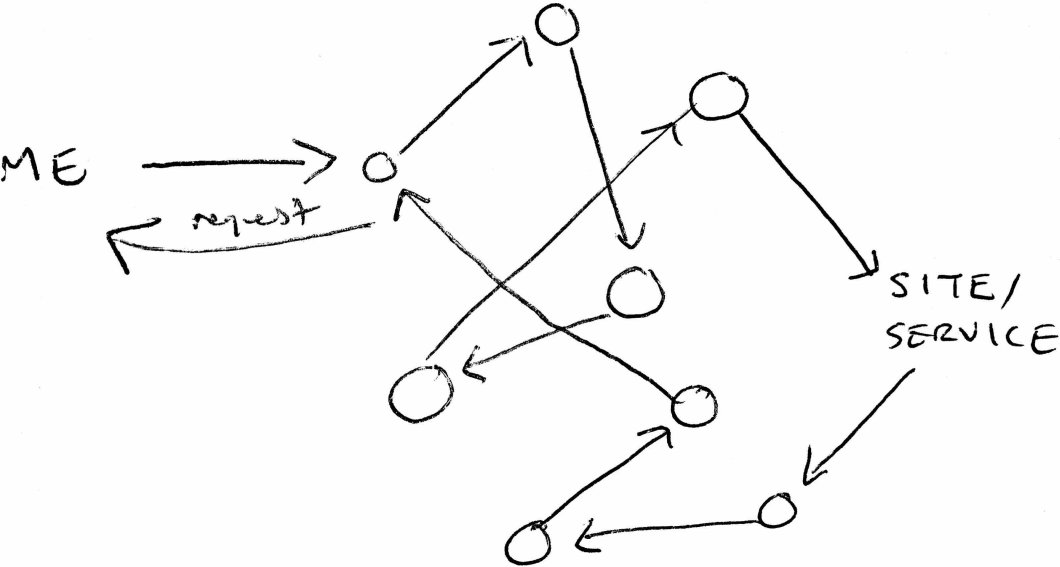
\includegraphics[width=\linewidth]{figures/p08-tor-sketch.jpg}
		\subcaption{Tor sketch.}
		\label{fig:p08-tor-sketch}
	\end{subfigure}
	\hfill
	\begin{subfigure}[t]{.45\linewidth}
		\centering
		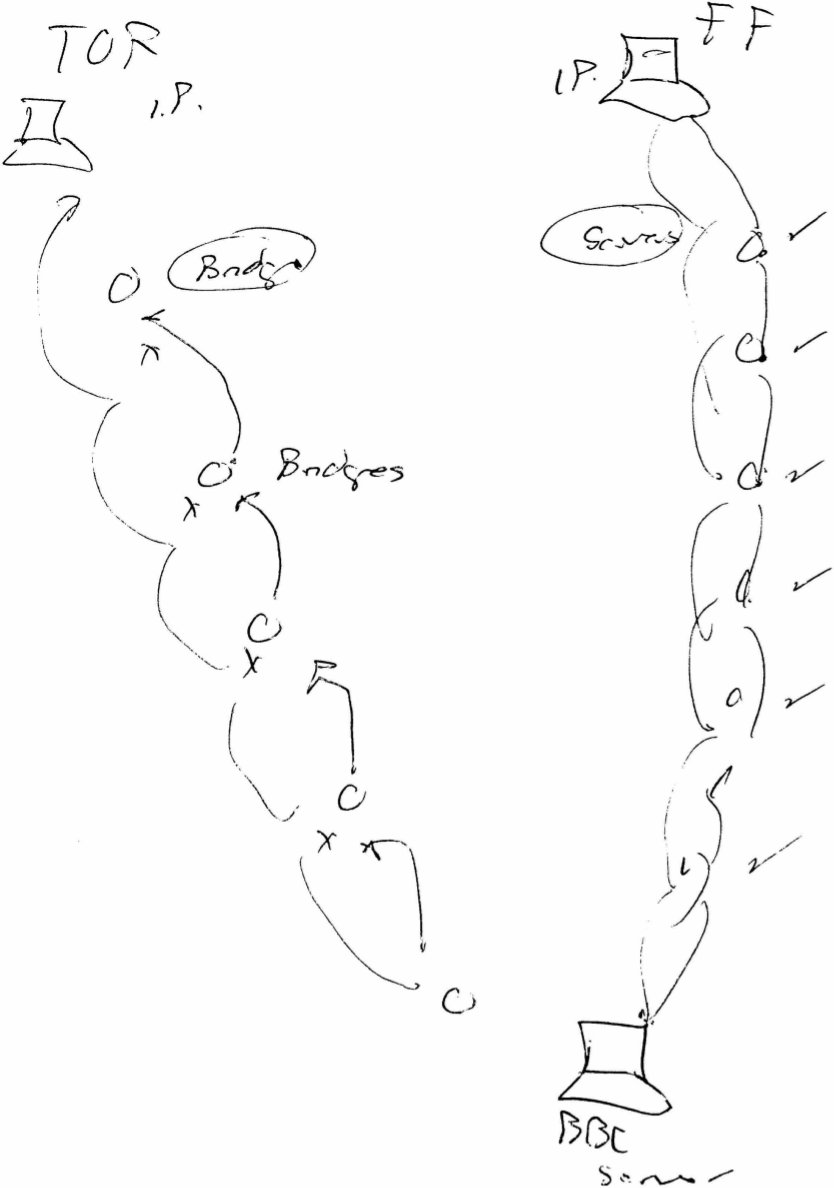
\includegraphics[width=.5\linewidth]{figures/p09-tor-sketch.jpg}
		\subcaption{Tor sketch.}
		\label{fig:p09-tor-sketch}
	\end{subfigure}

	\begin{subfigure}[t]{.45\linewidth}
		\centering
		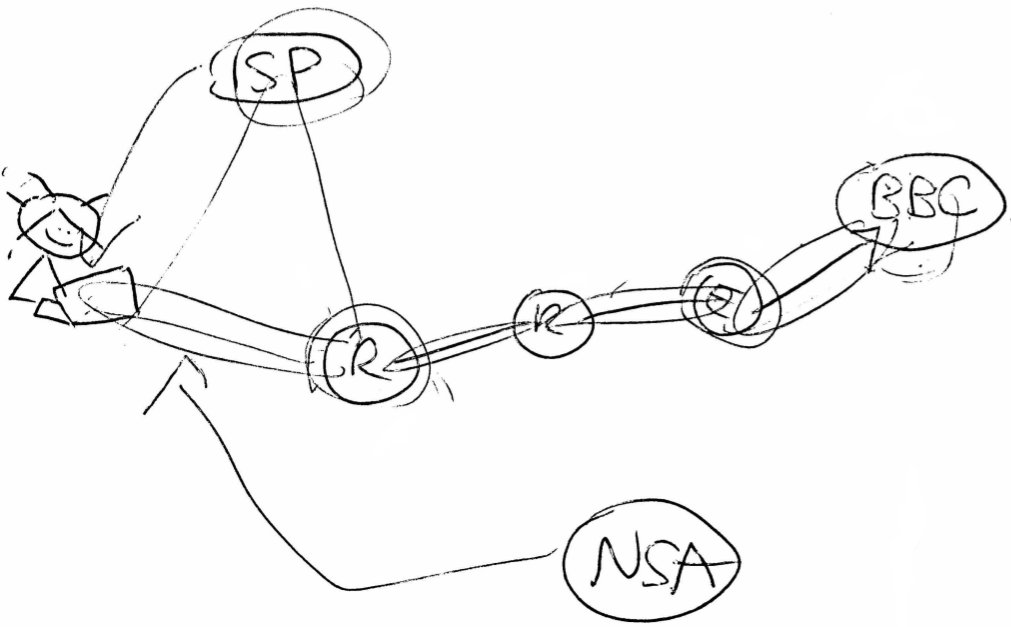
\includegraphics[width=\linewidth]{figures/p10-tor-sketch.jpg}
		\subcaption{Tor sketch.}
		\label{fig:p10-tor-sketch}
	\end{subfigure}
	\hfill
	\begin{subfigure}[t]{.45\linewidth}
		\centering
		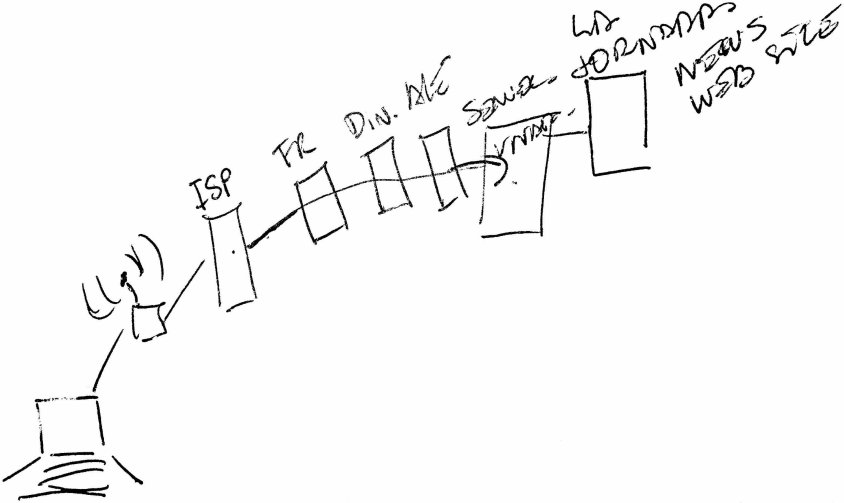
\includegraphics[width=\linewidth]{figures/p11-tor-sketch.jpg}
		\subcaption{Tor sketch.}
		\label{fig:p11-tor-sketch}
	\end{subfigure}

	\begin{subfigure}[t]{.45\linewidth}
		\centering
		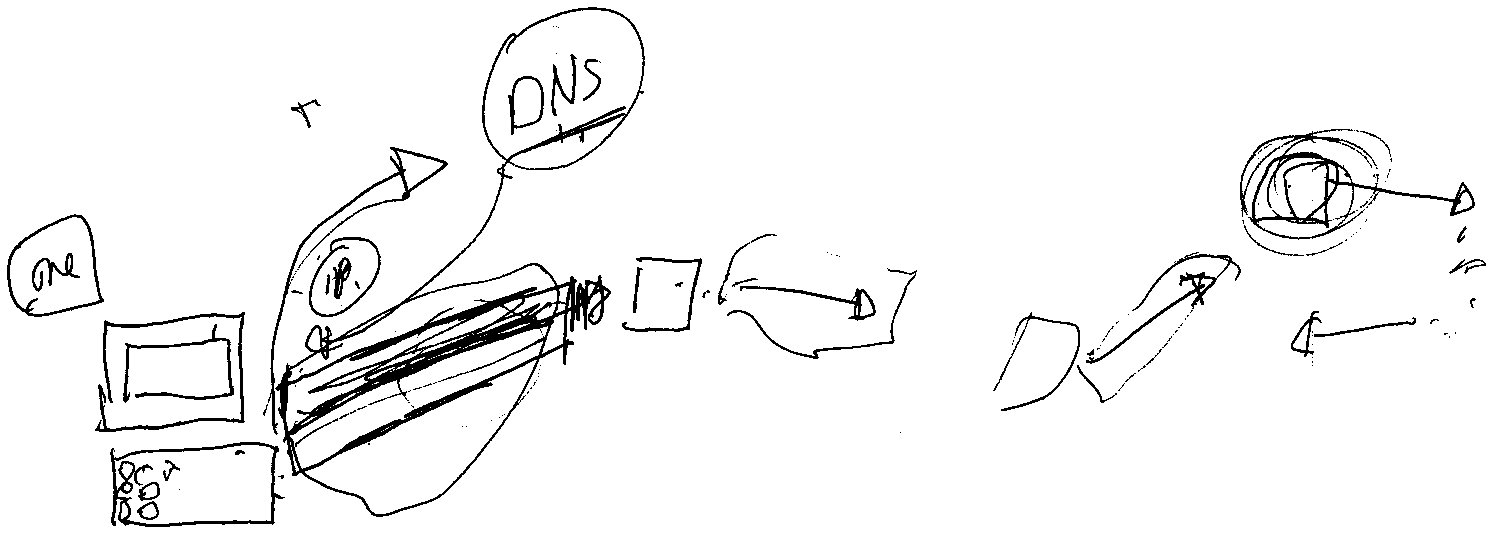
\includegraphics[width=\linewidth]{figures/p12-tor-sketch.jpg}
		\subcaption{Tor sketch.}
		\label{fig:p12-tor-sketch}
	\end{subfigure}
	\hfill
	\begin{subfigure}[t]{.45\linewidth}
		\centering
		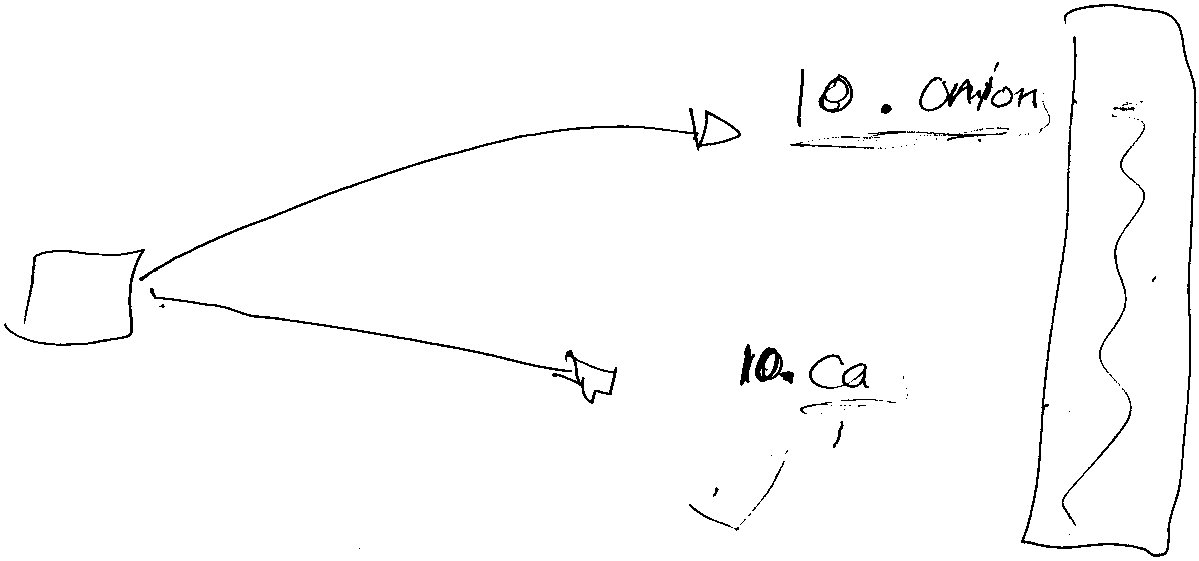
\includegraphics[width=\linewidth]{figures/p12-os-sketch.jpg}
		\subcaption{Onion service sketch.}
		\label{fig:p12-os-sketch}
	\end{subfigure}

	\caption{Bla.}
\end{figure*}

\begin{figure*}[ht]\ContinuedFloat
	\centering

	\begin{subfigure}[t]{.45\linewidth}
		\centering
		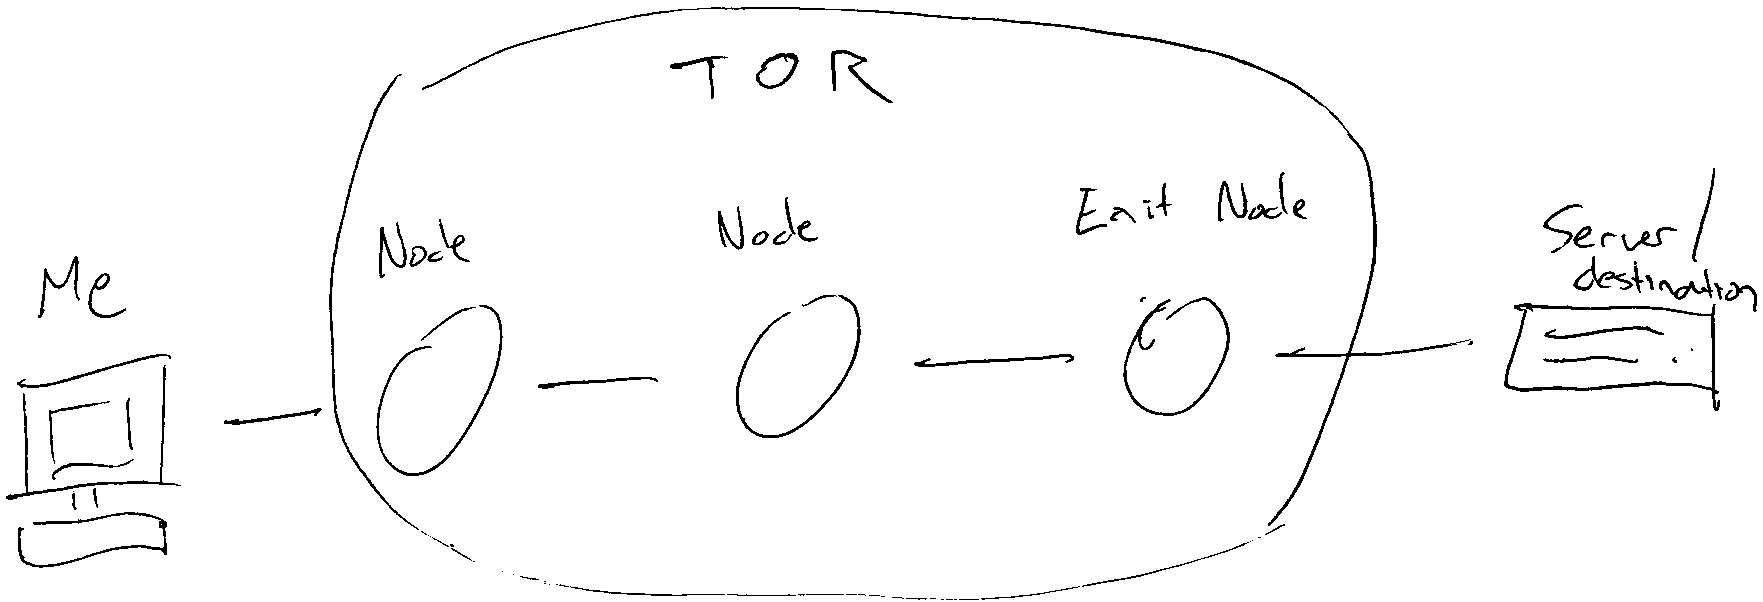
\includegraphics[width=\linewidth]{figures/p13-tor-sketch.jpg}
		\subcaption{Tor sketch.}
		\label{fig:p13-tor-sketch}
	\end{subfigure}
	\hfill
	\begin{subfigure}[t]{.45\linewidth}
		\centering
		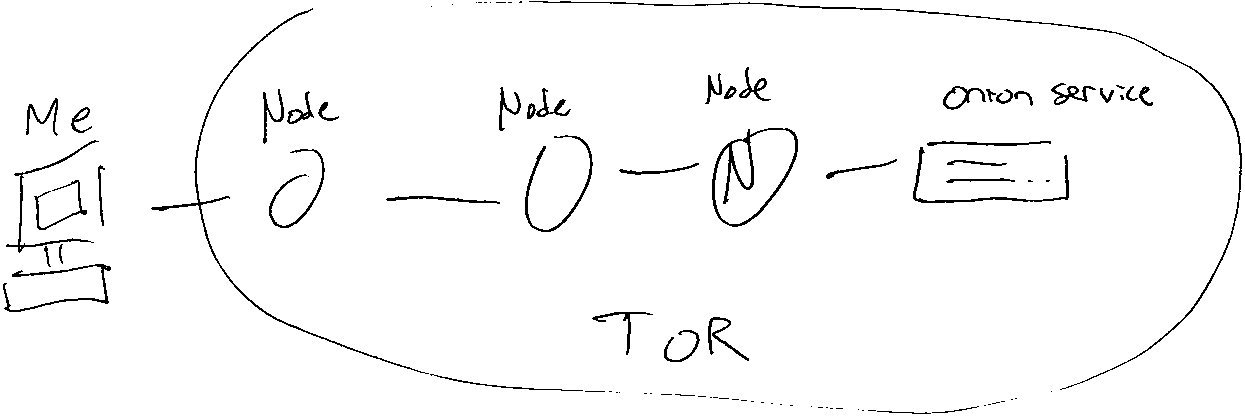
\includegraphics[width=\linewidth]{figures/p13-os-sketch.jpg}
		\subcaption{Onion service sketch}
		\label{fig:p13-os-sketch}
	\end{subfigure}

	\begin{subfigure}[t]{.45\linewidth}
		\centering
		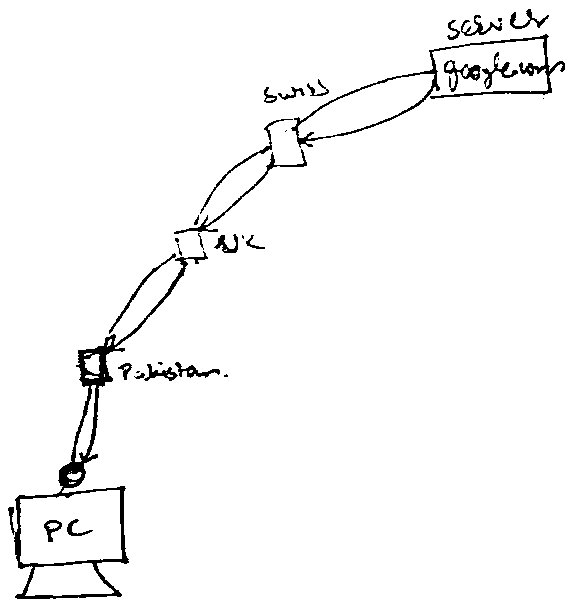
\includegraphics[width=.7\linewidth]{figures/p20-tor-sketch.jpg}
		\subcaption{Tor sketch.}
		\label{fig:p20-tor-sketch}
	\end{subfigure}
	\hfill
	\begin{subfigure}[t]{.45\linewidth}
		\centering
		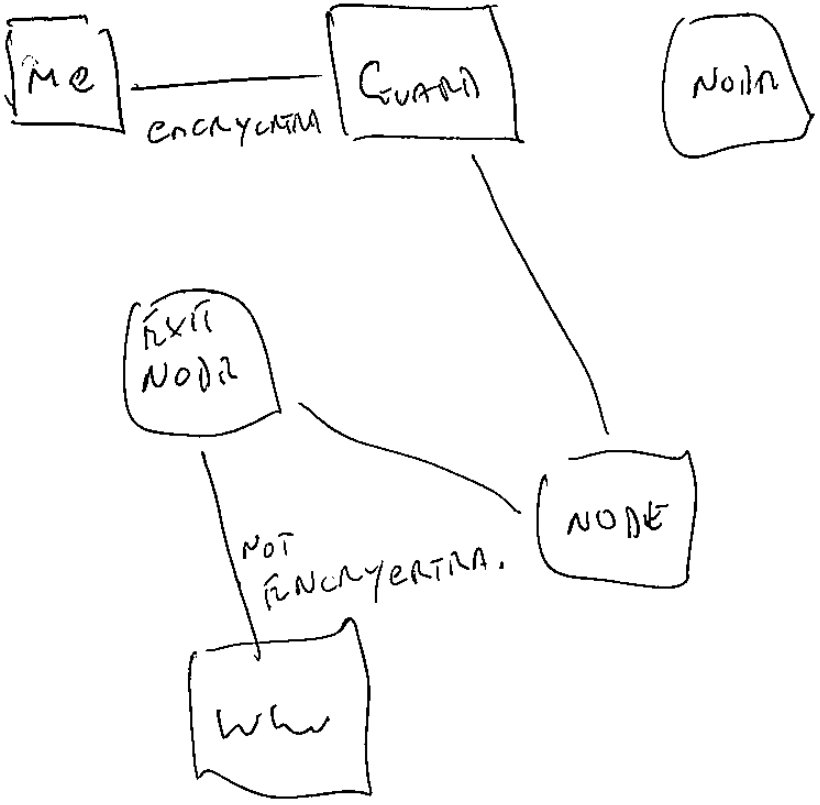
\includegraphics[width=.7\linewidth]{figures/p25-tor-sketch.jpg}
		\subcaption{Tor sketch.}
		\label{fig:p25-tor-skech}
	\end{subfigure}

	\begin{subfigure}[t]{.45\linewidth}
		\centering
		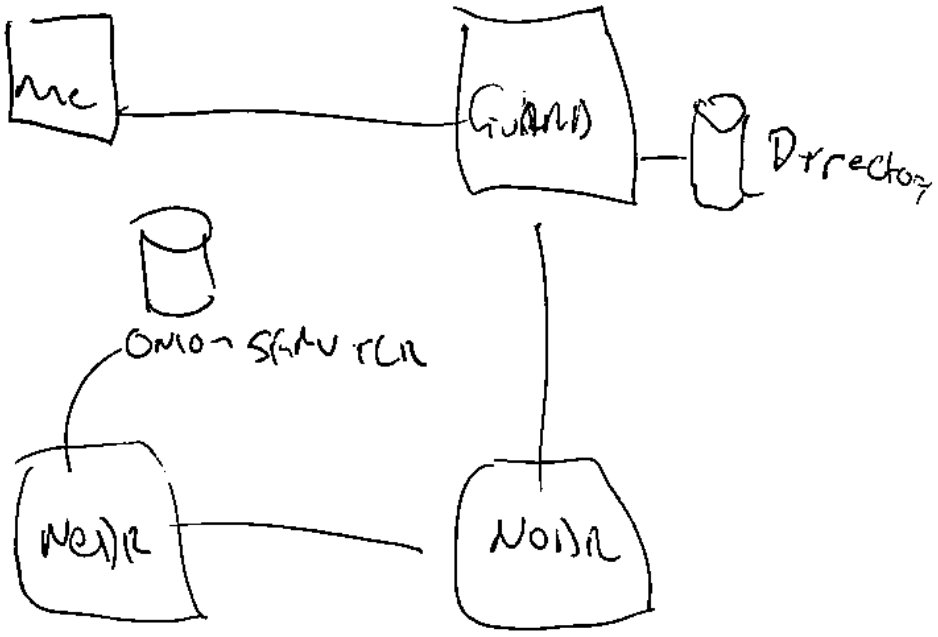
\includegraphics[width=\linewidth]{figures/p25-os-sketch.jpg}
		\subcaption{Onion service sketch.}
		\label{fig:p25-os-sketch}
	\end{subfigure}

	\caption{Bla.}
\end{figure*}

\subsection{Onion services}

\section{Pre-interview survey}
\label{sec:interview-survey}
We asked potential interview subjects to fill out a short survey (see below)
before we proceeded with selecting our subjects.  This survey allowed us to
select for subjects with the most interesting background.

\begin{enumerate}
    \item What is your name?
    \item What is your email address?
    \item Are you 18 years or older?
        \begin{itemize}[label=$\Circle$]
            \item Yes
            \item No
        \end{itemize}
    \item Have you used Tor Browser in the past?
        \begin{itemize}[label=$\Circle$]
            \item Yes
            \item No
        \end{itemize}
    \item Have you used onion services in the past?
        \begin{itemize}[label=$\Circle$]
            \item Yes
            \item No
        \end{itemize}
    \item How do you rate your knowledge about Internet privacy and security?
        \begin{itemize}[label=$\Circle$]
            \item Not at all knowledgeable
            \item Slightly knowledgeable
            \item Somewhat knowledgeable
            \item Moderately knowledgeable
            \item Extremely knowledgeable
        \end{itemize}
\end{enumerate}

\section{Interview questions}
\label{app:interview-questions}

We started the interview by handing our interviewees the consent form and
explained the purpose of our research to them.

\paragraph{Introductory questions}
\begin{enumerate}
    \item Tell us how often and why you use Tor?
    \item Do you remember the first time you used Tor?
\end{enumerate}

\paragraph{Expectations of privacy}
\begin{enumerate}
    \item What would make you use onion services more? (speed, quality/quantity
        of content, better domain format, popular websites having onion sites)
    \item Who or what are you trying to protect yourself against when using Tor?
    \item The domain format of onion sites is weird.  How do you deal with that?
    \item Would you like it if Tor Browser automatically redirected you to onion
        sites?  Even if that were the case for all onion sites?
    \item How do you learn about new onion sites?
    \item Do you think phishing is a concern with onion sites?  How do you know
        if an onion site is legitimate?
    \item Assume you use Tor to open \texttt{example.com}.  Who can see what?
        What if you open the corresponding onion site instead?
    \item What are you concerned about when using Tor?
    \item Certain things are hidden from certain entities when you are using
        Tor.  Please explain your beliefs.
    \item Some websites use ``vanity onion domains.''  Whare are your thoughts
        on that?
    \item Explain in your own words how you believe Tor works.
    \item Is there anything else about the usability of onion services that you
        wish to share?
\end{enumerate}

\section{Survey questions}
This section contains our online survey, consisting of seven sections.  Each
section holds a number of questions and their respective responses.  In the
responses, circles indicate that only one response can be selected while squares
indicate the possibility to select multiple responses.

\subsection{Demographic information}
\begin{enumerate}
    \item What is your gender?
        \begin{itemize}[label=$\Circle$]
            \item Female
            \item Male
            \item Other
        \end{itemize}

    \item What is your age?
        \begin{itemize}[label=$\Circle$]
            \item 18--25 years
            \item 26--35 years
            \item 36--45 years
            \item 46--55 years
            \item 56--65 years
            \item Older than 65 years
        \end{itemize}

    \item What is the highest level of education that you completed?
        \begin{itemize}[label=$\Circle$]
            \item Some education, but no high school diploma or equivalent
            \item High school diploma or equivalent
            \item College or university degree (for example a bachelor's degree)
            \item Post-graduate education (for example a master's or a doctorate degree)
        \end{itemize}

    \item How would you rate your knowledge about Internet privacy and security?
        \begin{itemize}[label=$\Circle$]
            \item No knowledge
            \item Mildly knowledgeable
            \item Moderately knowledgeable
            \item Highly knowledgeable
            \item Expert
        \end{itemize}
\end{enumerate}

\subsection{Tor usage}
\begin{enumerate}
    \item Tor Browser is a web browser---similar to Firefox---that allows you
        to browse the web anonymously. Have you ever used Tor Browser?
        \begin{itemize}[label=$\Circle$]
            \item Yes
            \item No
        \end{itemize}

    \item How frequently do you use Tor Browser?\\(Please select the answer
        that applies the most.)
        \begin{itemize}[label=$\Circle$]
            \item Never
            \item On average less than once a month
            \item On average about once a month
            \item On average about once a week
            \item On average about once a day
            \item Tor Browser is my main browser
        \end{itemize}

    \item When using Tor Browser, who do you want to protect your browsing
        activity from?\\(Check all that apply.)
        \begin{itemize}[label=$\Square$]
            \item My government
            \item Other governments
            \item My Internet service provider (ISP)
            \item My school
            \item My employer
            \item Friends and family
            \item Advertising companies
            \item Hackers in open WiFis (for example in coffee shops)
            \item Other (Please elaborate below.)
        \end{itemize}

    \item For quality purposes, please select only ``iPhone'' and ``Android''
        in the options below.
        \begin{itemize}[label=$\Square$]
            \item PC
            \item Mac
            \item iPhone
            \item Android
            \item Other (Please elaborate below.)
        \end{itemize}
\end{enumerate}

\subsection{Onion site usage}
\begin{enumerate}
    \item The Tor Browser allows you to browse ``onion sites.'' Onion sites are
        web sites that can only be accessed over the Tor network. The domains of
        onion sites end with \texttt{.onion} instead of \texttt{.com},
        \texttt{.net}, etc.; they are of constant length; and they tend to
        ``look random.'' For example, The Tor Project's web site,
        \texttt{torproject.org}, is also available at
        \texttt{expyuzz4wqqyqhjn.onion} as an onion site.

    \item How frequently do you use Tor Browser to browse onion sites?\\(Please
        select the answer that applies the most.)
        \begin{itemize}[label=$\Circle$]
            \item I have never used onion sites
            \item On average less than once a month
            \item On average about once a month
            \item On average about once a week
            \item On average about once a day
        \end{itemize}

    \item How frequently do you use onion sites for purposes other than web
        browsing? For example for remote login (SSH) or chat (IRC, or XMPP)?
        \begin{itemize}[label=$\Circle$]
            \item Never
            \item On average less than once a month
            \item On average about once a month
            \item On average about once a week
            \item On average about once a day
        \end{itemize}

    \item Why do you browse onion sites?\\(Check all that apply.)
        \begin{itemize}[label=$\Square$]
            \item Because of the additional anonymity -- traffic to onion sites
                never leaves the Tor network
            \item Because of the additional security -- onion sites provide
                end-to-end security
            \item Some sites I like are only available as onion sites and not
                as normal web sites
            \item No particular reason; I occasionally just click on links to
                onion sites
            \item I read about the ``dark web'' and wanted to form my own
                opinion
            \item Other (Please elaborate below.)
        \end{itemize}

    \item How do you discover new onion sites?\\(Check all that apply.)
        \begin{itemize}[label=$\Square$]
            \item I browse the list of onion site search engines such as
                \texttt{ahmia.fi}
            \item From social networking sites such as Reddit or Twitter
            \item Recommendations from friends and family
            \item I randomly encounter them while browsing the web
            \item I am not interested in learning about new onion sites
            \item Other (Please elaborate below.)
        \end{itemize}

    \item Are you satisfied with the way you discover new onion sites?\\(Check
        all that apply.)
        \begin{itemize}[label=$\Circle$]
            \item Yes
            \item No (Please elaborate below.)
        \end{itemize}

    \item Many people memorize popular domains such as \texttt{youtube.com} and
        \texttt{wikipedia.com} for quick access. How do you deal with the domain
        of onion sites such as \texttt{expyuzz4wqqyqhjn.onion}?\\(Check all that
        apply.)
        \begin{itemize}[label=$\Square$]
            \item I save a list of onion domains in a file on my computer
            \item I write onion domains down using pen and paper
            \item I bookmark onion domains in Tor Browser
            \item I use a web-based bookmarking service such as Firefox Sync or
                Google Bookmarks
            \item I use a search engine each time (for example, to search for
                ``facebook onion site'')
            \item I go to web pages I trust that have links to onion sites
            \item I memorize some onion domains
            \item I don't have a good solution
            \item Other (Please elaborate below.)
        \end{itemize}

    \item The Tor Project is currently working on the next generation of onion
        services. The new onion domain format will consist of 52 characters,
        for example:
        \texttt{a1uik0w1gmfq3i5ievxdm9ceu27e88g6o7pe0rffdw9jmn\-twkdsd.onion}
        Do you expect this to change your browsing habits?
        \begin{itemize}[label=$\Circle$]
            \item Yes (Please elaborate below.)
            \item No (Please elaborate below.)
        \end{itemize}

    \item Do you have a Facebook account?
        \begin{itemize}[label=$\Circle$]
            \item Yes
            \item No
        \end{itemize}

    \item Have you ever logged in to Facebook over its onion site
        \texttt{facebookcorewwwi.onion}?
        \begin{itemize}[label=$\Circle$]
            \item Yes, that is the only way I log in to Facebook
            \item Yes, occasionally
            \item No, never
            \item I didn't know about this onion site until now
        \end{itemize}

    \item For quality purposes, please select ``Yes, more than once'' in the
        options below.
        \begin{itemize}[label=$\Circle$]
            \item Yes, once
            \item Yes, more than once
            \item No
        \end{itemize}

    \item How many onion domains do you have fully memorized?
        \begin{itemize}[label=$\Circle$]
            \item None
            \item One
            \item Two
            \item Three
            \item Four
            \item More than four
        \end{itemize}

    \item Is \texttt{facebookcorewwwi.onion} among the sites that you have
        memorized?
        \begin{itemize}[label=$\Circle$]
            \item Yes
            \item No
        \end{itemize}

    \item Why do you memorize onion domains?\\(Check all that apply.)
        \begin{itemize}[label=$\Square$]
            \item It allows me to open the site more quickly
            \item I don't want to leave any digital traces of the onion sites I
                visit
            \item That way I can be sure that I end up at the right onion site
                and not a phishing site
            \item After typing a domain many times, I automatically start to
                memorize it
            \item Other (Please elaborate below.)
        \end{itemize}

    \item Imagine you had to memorize onion domains. Please rate the difficulty
        of memorizing the following domains.
        \begin{itemize}
            \item \texttt{facebookcorewwwi.onion}
            \item \texttt{expyuzz4wqqyqhjn.onion}
            \item \texttt{torproz4wqqyqhjn.onion}
            \item \texttt{torprojectqyqhjn.onion}
        \end{itemize}
        For each answer, we provided the following Likert scale:
        \begin{itemize}
            \item Very easy
            \item Somewhat easy
            \item Neither easy nor difficult
            \item Somewhat difficult
            \item Very difficult
        \end{itemize}

    \item Please explain the reason for the rating you gave above.

    \item If popular web sites such as YouTube, Twitter, or Amazon offered
        onion sites in parallel to their normal web sites, which one would you
        prefer?
        \begin{itemize}[label=$\Circle$]
            \item Always the normal web site
            \item Always the onion site
            \item Other (Please elaborate below.)
        \end{itemize}

    \item Please explain the reason for the choice you made above.

    \item If Tor Browser could automatically redirect you from a web site to
        its corresponding onion site (for example from \texttt{facebook.com} to
        \texttt{facebookcorewwwi.onion}), would you use this feature?
        \begin{itemize}[label=$\Circle$]
            \item No, never
            \item Yes, for some sites
            \item Yes, always
            \item Other (Please elaborate below.)
        \end{itemize}

    \item Please explain the reason for the choice you made above.

    \item Please rate how important the following criteria are for the
        usability of onion sites.\\(Check all that apply.)
        \begin{itemize}
            \item Page load time
            \item Quality of content (e.g., up-to-date, interesting sites)
            \item Diversity of content (e.g., sites about politics, technology, social media, etc.)
            \item Easy-to-remember domain format
            \item Having an onion service version of popular services such as Facebook
            \item Existence of a search engine (like Google) for onion services
        \end{itemize}
        For each answer, we provided the following Likert scale:
        \begin{itemize}
            \item Very unimportant
            \item Somewhat unimportant
            \item Neutral
            \item Somewhat important
            \item Very important
        \end{itemize}
\end{enumerate}

\subsection{Onion site operation}
\begin{enumerate}
    \item Have you ever set up your own onion site?
        \begin{itemize}[label=$\Circle$]
            \item Yes
            \item No, but I have considered doing it
            \item No, and I have not considered it
        \end{itemize}

    \item Did you experience any issues while setting up your onion site?
        \begin{itemize}[label=$\Circle$]
            \item No
            \item Yes (Please elaborate below.)
        \end{itemize}

    \item Why did you set up your own onion site?\\(Check all that apply.)
        \begin{itemize}[label=$\Square$]
            \item I wanted my site to be anonymous
            \item I wanted my site to have end-to-end security
            \item I used a tool that automatically creates onion sites (for
                example OnionShare or Ricochet)
            \item To make my site accessible behind a NAT device
            \item Out of curiosity
            \item Other (Please elaborate below.)
        \end{itemize}

    \item Were the onion site(s) you set up intended for the general public, or
        only for private use?\\(Check all that apply.)
        \begin{itemize}[label=$\Square$]
            \item For public use (for example, a public blog)
            \item For private use (for example, sharing pictures with a friend)
        \end{itemize}

    \item Please rate the level of concern you would have for the following
        scenarios.
        \begin{itemize}
            \item Somebody deanonymizing my onion service
            \item Somebody taking my onion service offline
            \item Somebody setting up a phishing site targeting my onion service
        \end{itemize}
        For each answer, we provided the following Likert scale:
        \begin{itemize}
            \item Not at all concerned
            \item Slightly concerned
            \item Somewhat concerned
            \item Moderately concerned
            \item Extremely concerned
        \end{itemize}
\end{enumerate}

\subsection{Onion site phishing and impersonation}
\begin{enumerate}
    \item Did you ever type an onion domain manually?
        \begin{itemize}[label=$\Circle$]
            \item Yes
            \item No
        \end{itemize}

    \item Please elaborate on why you typed an onion domain manually?

    \item How do you realize that you made a typo when typing an onion
        URL?\\(Check all that apply.)
        \begin{itemize}[label=$\Square$]
            \item When the page won't load
            \item When a wrong page shows up
            \item I don't know
            \item Other (Please elaborate below.)
        \end{itemize}

    \item Have you ever thought about whether the onion site you are browsing
        is the authentic site you are trying to reach?
        \begin{itemize}[label=$\Circle$]
            \item Yes
            \item No
        \end{itemize}

    \item How do you know an onion site is the legitimate site you are trying
        to reach, and not an impersonation?\\(Check all that apply.)
        \begin{itemize}[label=$\Square$]
            \item I verify (part of) the onion domain in Tor Browser's address
                bar
            \item I use bookmarks when accessing onion sites
            \item I go to the corresponding web site and look for the link to
                its onion site
            \item Sometimes I cannot tell the difference between the legitimate
                and the impersonation site
            \item I copy\&paste onion domains from a trusted source
            \item I check if the onion site's HTTPS certificate is valid (if it
                has one)
            \item I don't check
            \item Other (Please elaborate below.)
        \end{itemize}

    \item How many characters of a domain do you verify? Recall that an onion
        domain has 16 characters.
        \begin{itemize}[label=$\Circle$]
            \item 1--3
            \item 4--6
            \item 7--9
            \item 10--12
            \item 13--16
        \end{itemize}

    \item For quality purposes, please select ``Less than once a month'' in the
        options below.
        \begin{itemize}[label=$\Circle$]
            \item Less than once a month
            \item About once a month
            \item About once a week
            \item About once a day
        \end{itemize}

    \item Have you ever sent Bitcoins to a Bitcoin address that you got from an
        onion site?
        \begin{itemize}[label=$\Circle$]
            \item Yes
            \item No
        \end{itemize}

    \item Some onion site owners use tools to have a short word at the
        beginning of their onion domain. This is why Facebook's domain
        (\texttt{facebookcorewwwi.onion}) looks the way it does. We call these
        customized domains ``vanity onion domains.''

    \item What is your overall opinion on vanity onion domains?\\(Check all
        that apply.)
        \begin{itemize}[label=$\Square$]
            \item I find them useful because they are easier to memorize
            \item I find them useful because they are easier to recognize
            \item I like them because they make an onion site look ``unique''
            \item I dislike them because onion sites shouldn't contain their
                name in their domain
            \item I don't see a benefit
            \item I don't have an opinion
            \item Other (Please elaborate below.)
        \end{itemize}
\end{enumerate}

\subsection{Expectations of privacy}
\begin{enumerate}
    \item Let us move away from onion services and turn to expectations of
        privacy. If you use Tor Browser to open \texttt{http://example.com}, who
        do you believe can see your connection to
        \texttt{http://example.com}?\\(Check all that apply.)
        \begin{itemize}[label=$\Square$]
            \item Your Internet service provider (ISP)
            \item The ISP of \texttt{example.com}
            \item Your Tor ``exit relay''
            \item Your Tor ``guard relay''
            \item Nobody
            \item I don't know
            \item Other (Please elaborate below.)
        \end{itemize}

    \item Now imagine that you are instead using Tor Browser to open the
        \emph{onion site} of \texttt{http://example.com}. Who do you believe can
        see your connection to this onion site?\\(Check all that apply.)
        \begin{itemize}[label=$\Square$]
            \item Your Internet service provider (ISP)
            \item The ISP of the onion site
            \item Your Tor ``exit relay''
            \item Your Tor ``guard relay''
            \item The ``guard relay'' of the onion site
            \item Nobody
            \item I don't know
            \item Other (Please elaborate below.)
        \end{itemize}

    \item How safe do you feel when using Tor Browser compared to another
        browser?
        \begin{itemize}[label=$\Circle$]
            \item Very unsafe
            \item Somewhat unsafe
            \item Neutral
            \item Somewhat safe
            \item Very safe
        \end{itemize}

    \item Please elaborate on why you feel that way when using Tor Browser.

    \item Please tell us about how safe you feel when browing onion sites as
        compared to normal websites?
        \begin{itemize}[label=$\Circle$]
            \item Very unsafe
            \item Somewhat unsafe
            \item Neutral
            \item Somewhat safe
            \item Very safe
        \end{itemize}

    \item Please elaborate on why you feel that way when using onion sites.

    \item For quality purposes, please select only ``Very unsafe'' in the options
        below.
        \begin{itemize}[label=$\Circle$]
            \item Very unsafe
            \item Somewhat unsafe
            \item Neutral
            \item Somewhat safe
            \item Very safe
        \end{itemize}

    \item Assume you just set up your own onion site. Who do you believe can
        see that this onion site was set up?\\(Check all that apply.)
        \begin{itemize}[label=$\Square$]
            \item The onion site's ISP
            \item The developers of The Tor Project
            \item (Some) Tor relays
            \item Nobody
            \item I don't know
            \item Other (Please elaborate below.)
        \end{itemize}

    \item Facebook already runs the onion site \texttt{facebookcorewwwi.onion}.
        How difficult or easy do you believe is it for someone to create domains
        that begin with the following characters? Note that the {\color{red}
        \texttt{X}} symbols below
        are just placeholders. What matters is the first characters.
        \begin{itemize}
            \item \texttt{facebookcore\textcolor{red}{XXXX}.onion}
            \item \texttt{facebook\textcolor{red}{XXXXXXXX}.onion}
            \item \texttt{face\textcolor{red}{XXXXXXXXXXXX}.onion}
        \end{itemize}
        For each answer, we provided the following Likert scale:
        \begin{itemize}
            \item Very easy
            \item Moderately easy
            \item Neither easy nor difficult
            \item Moderately difficult
            \item Very difficult
            \item I don't know
        \end{itemize}
\end{enumerate}

\subsection{End of survey}
\begin{enumerate}
    \item Finally, is there anything else about the usability of Tor or onion
        services that you wish to share with us?
\end{enumerate}

\subsection{Coding themes}
\label{sec:coding-themes}

\begin{table*}[ht]
	\centering
	\caption{The codewords we developed while coding our interviews, together
	with their respective explanations, and the number of interviewees who
	brought them up.}

	\label{tab:tor-sketches}

	\begin{tabular}{l l l r}
	\toprule
	Category & Codeword & Explanation & Occurences \\
	\midrule

	& 90s-experience & Tor provides a browsing experience akin to the 90s. & N \\
	& slow-browsing & Browsing the web over Tor feels slow. & N \\
	& empowerment & Tor equips users with control over their browsing. & N \\

	\bottomrule
	\end{tabular}
\end{table*}
